	\begin{figure*}[htb]
	\begin{minipage}[h]{0.30\linewidth}
		\centering
		\centerline{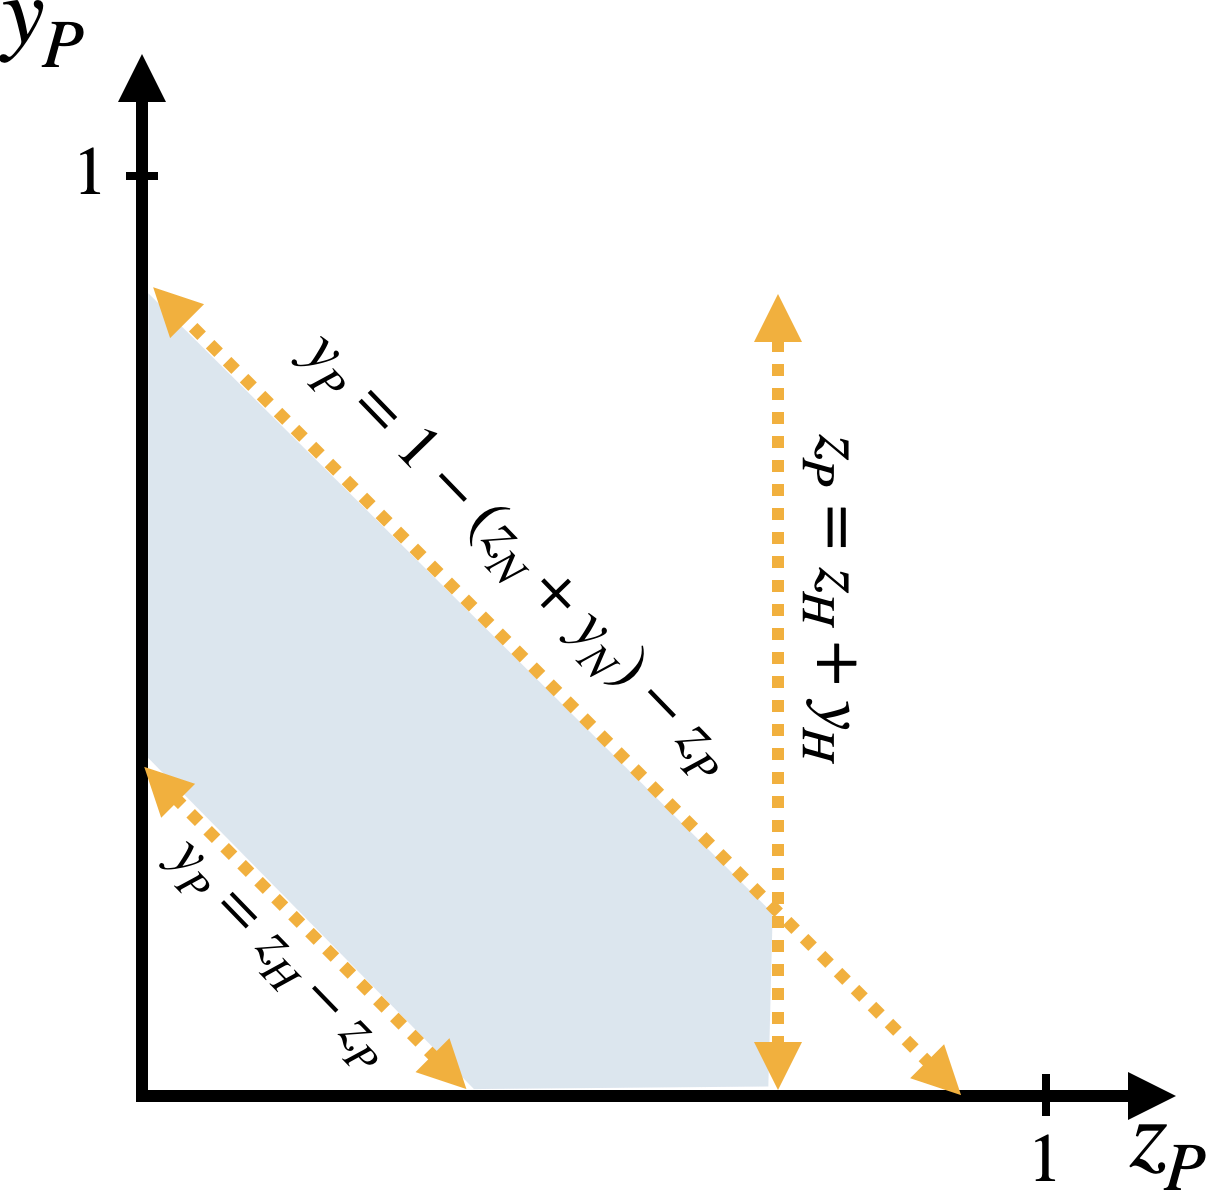
\includegraphics[width=4.0cm]{figs/parent_region.png}}
		\centerline{(a)}\medskip
		%  \vspace{2.0cm}
	\end{minipage}
	%
	\begin{minipage}[h]{.30\linewidth}
		\centering
		\centerline{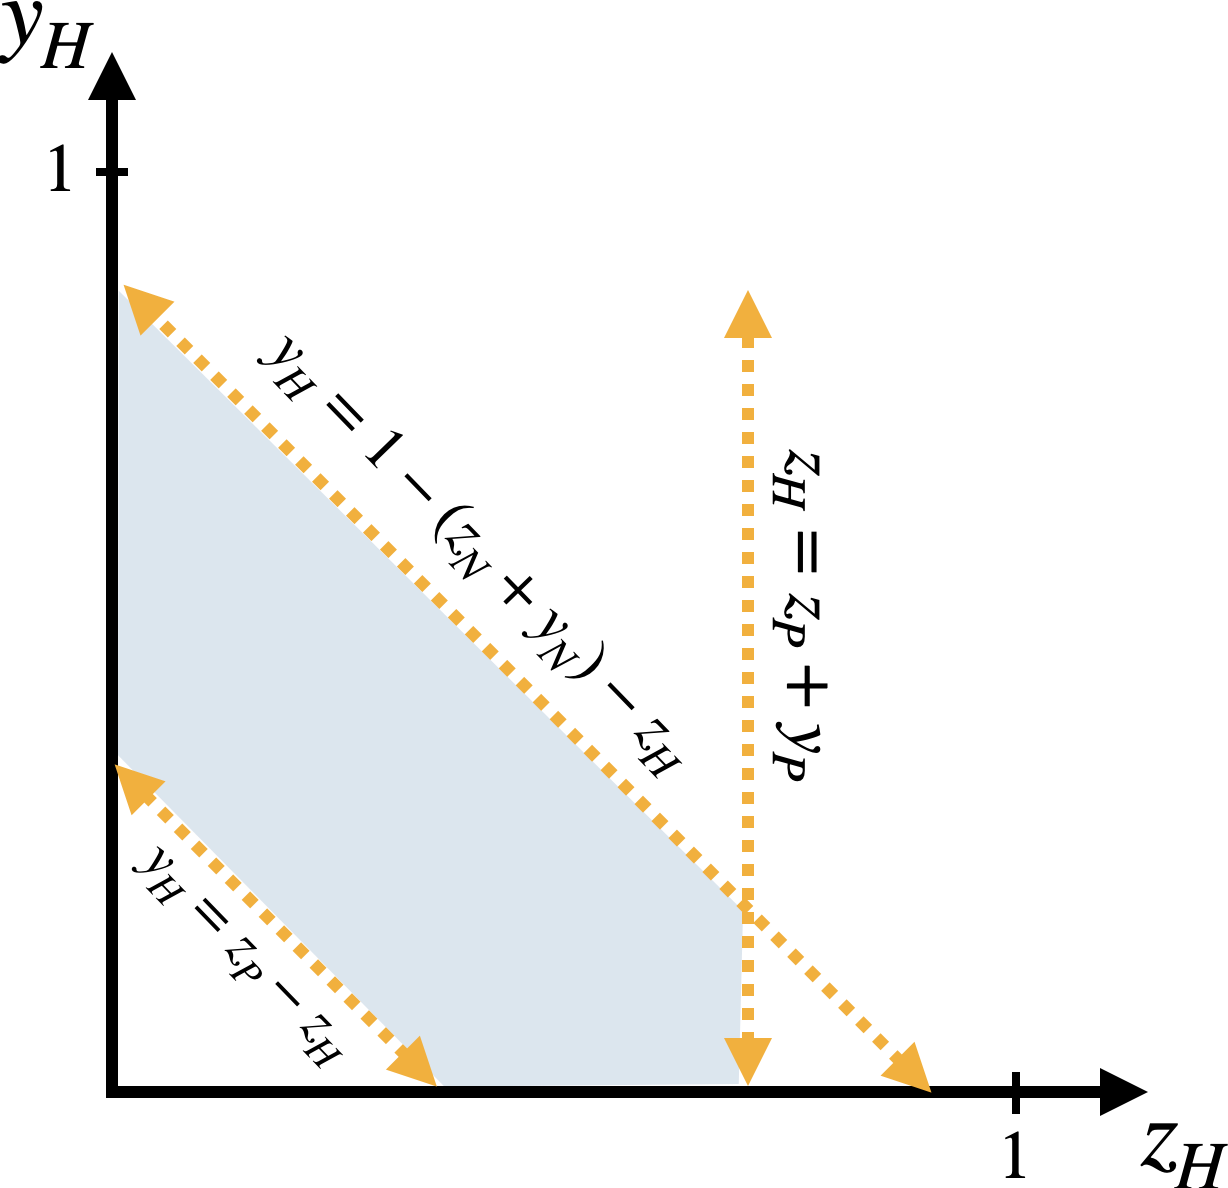
\includegraphics[width=4.0cm]{figs/inherited_region.png}}
		%  \vspace{1.5cm}
		\centerline{(b)}\medskip
	\end{minipage}
	%	\hfill
	\begin{minipage}[h]{0.30\linewidth}
		\centering
		\centerline{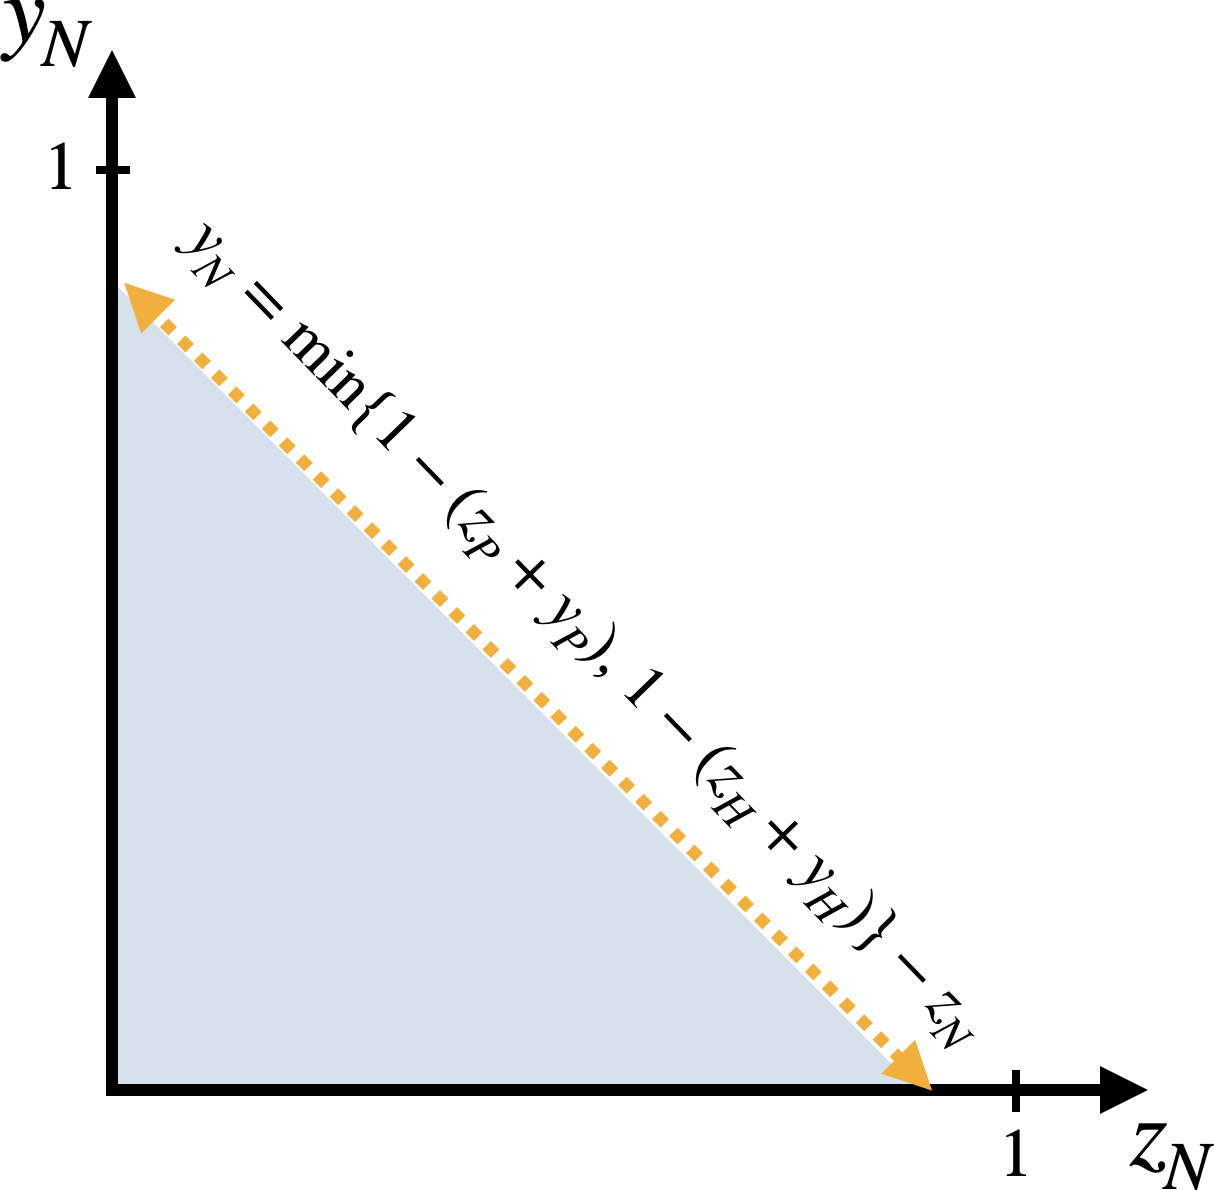
\includegraphics[width=4.0cm]{figs/novel_region.png}}
		%  \vspace{1.5cm}
		\centerline{(c) }\medskip
	\end{minipage}
	%
	\caption{The feasible set is shown above by the shaded region for each step of the proposed block-coordinate descent approach. (a) In Step 1, we obtain the solution for the parent's variables $\zP$ and $\yP$ given fixed child inherited and novel indicator variables $\zH, \zN, \yH, \text{and } \yN$. (b), (c) In Step 3, we obtain the solution for the child's variables.  }
	\label{fig:regions}
	%
\end{figure*}
We propose solving our problem using an alternating block-coordinate descent approach, following the methods used in previous work \cite{MB_diploidTrios, lazar_2021,MB_SingleParentDiploid}. For this,  we fix all but one individual and solve (\ref{subproblemIterate}) over both indicator variables for that individual. We continue successively minimizing both indicator variables for each individual while the other individuals are fixed. The feasible region for this step is illustrated in \ref{fig:regions}.\\


\noindent \textbf{Step 0:} We begin by computing the unconstrained minimizer of (\ref{subproblemIterate}), which is given by $\vec{f} = \vec{r}^{\,k} - \frac{\tau}{\alpha_k}\gamma\mathbf{1}$. % not this. it is something like 1/alpha[tau; tau; tau*gamma; tau; tau; tau*gammas]
Next,  we initialize the child's inherited and novel indicator variables by applying the following rule:
\begin{equation*}
	\begin{aligned}
		\hat{z}_H^{(0)} = \{0,r_{z_H}^k - \frac{\tau}{\alpha_k},1 \}, & \quad \hat{z}_N^{(0)} = \{0,r_{z_N}^k - \frac{\tau}{\alpha_k}\gamma,1 \},\\
		\hat{y}_H^{(0)} = \{0,r_{y_H}^k - \frac{\tau}{\alpha_k},1 \}, &
		\quad \hat{y}_N^{(0)} = \{0,r_{y_N}^k - \frac{\tau}{\alpha_k}\gamma,1 \}
	\end{aligned}
\end{equation*}
Further, if $\hat{z}_H^{(0)} + \hat{y}_H^{(0)}>1$, then we let $\hat{z}_H^{(0)} = \hat{y}_H^{(0)} = 0.5$. We adjust $\hat{z}_N^{(0)}$ and $\hat{y}_N^{(0)}$ similarly. We apply these rules to ensure our initialization is consistent with the set of feasible solutions. To initialize the parent indicator variables, we let $\hat{z}_P^{(0)} = r_{z_P}^k - \frac{\tau}{\alpha_k}$ and $\hat{y}_P^{(0)} = r_{y_P}^k - \frac{\tau}{\alpha_k}$. 
We initialize the index with $i=1$. \\

\noindent \textbf{Step 1:} Once we have obtained estimates for child's inherited and novel diploid indicator variables, $\hat{z}_H^{(i-1)}, \hat{y}_H^{(i-1)}, \hat{z}_N^{(i-1)}, \hat{y}_N^{(i-1)}$, from the previous iteration, we project $\hat{z}_P^{(i-1)}$ and $\hat{y}_P^{(i-1)}$ onto the feasible set $S$ with fixed inherited and novel variables to obtain the new parent indicator values $\hat{z}_P^{(i)}$ and $\hat{y}_P^{(i)}$. This projection is similar to the projections done in \cite{MB_SingleParentDiploid, MB_diploidTrios}. \\

\noindent \textbf{Step 2:} After obtaining the new estimates for the parent diploid indicator variables $\hat{z}_P^{(i)}$ and $\hat{y}_P^{(i)}$ from Step 1, we project $\hat{z}_H^{(i-1)}, \hat{y}_H^{(i-1)}$ onto our feasible set $S$ with fixed parent and child's novel indicator variables to obtain the new child's inherited indicator variables $\hat{z}_H^{(i)}$ and $\hat{y}_H^{(i)}$.\\ 

\noindent \textbf{Step 3:} After obtaining the new estimates for the child's inherited diploid indicator variables $\hat{z}_H^{(i)}$ and $\hat{y}_H^{(i)}$ from Step 2, we project $\hat{z}_N^{(i-1)}, \hat{y}_N^{(i-1)}$ onto our feasible set $S$ with fixed parent and child's inherited indicator variables to obtain the new child's novel indicator variables $\hat{z}_N^{(i)}$ and $\hat{y}_N^{(i)}$. \\

We repeat Steps 1, 2, and 3 until some convergence criteria are satisfied. Steps 1 and 2  result in identical feasible regions. 